\section{Watchdog timer}
\label{sec:wdt}
\pulpissimo features a Watchdog timer.


\begin{figure}[H]
  \centering
  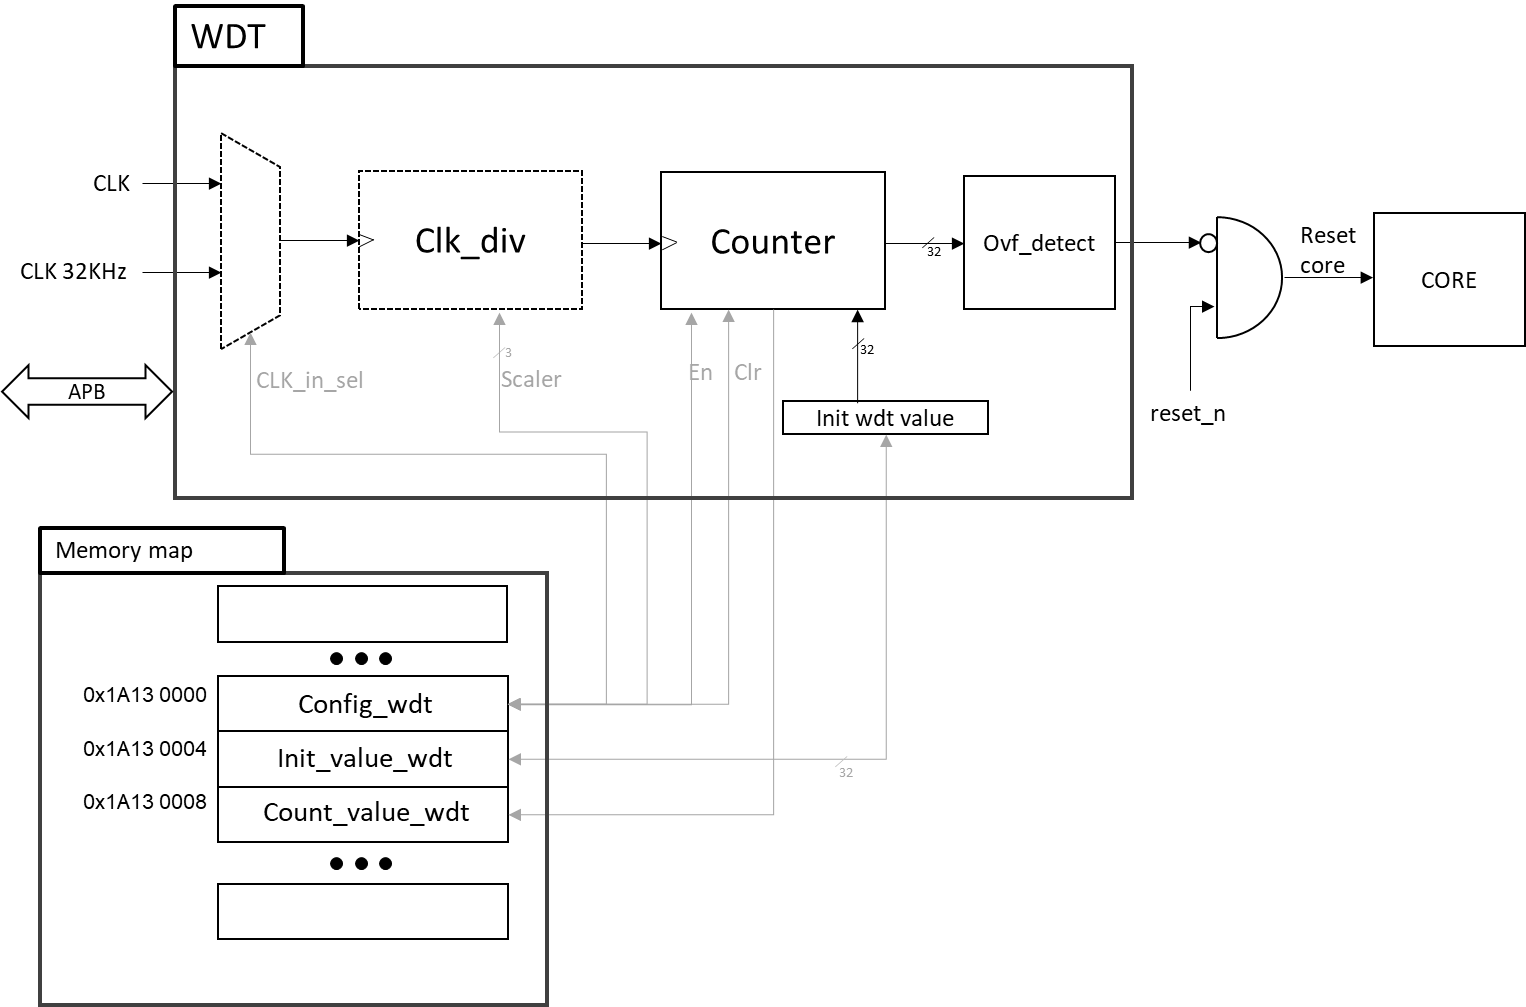
\includegraphics[width=0.9\textwidth]{./figures/wdt.png}
  \caption{WDT block diagram.}
  \label{fig:wdt_overview}
\end{figure}


The following registers can be accessed.

\regDesc{0x1A13\_0000}{0x0000\_0000}{Config wdt}{
  \begin{bytefield}[rightcurly=.,endianness=big]{32}
  \bitheader{31,30,29,28,27,26,25,24,23,22,21,20,19,18,17,16,15,14,13,12,11,10,9,8,7,6,5,4,3,2,1,0} \\
  \begin{rightwordgroup}{CONF}
    \bitbox{26}{- - -}
    \bitbox{1}{\tiny Clk}
    \bitbox{3}{\tiny Presc}
    \bitbox{1}{\tiny Clr}
    \bitbox{1}{\tiny En}
  \end{rightwordgroup}\\
  \end{bytefield}
}{
  \regItem{R/W register}{}{
	CONF reg bit
    \begin{itemize}
      \item \signal{Bit 0 :} EN (Enable watchdog timer)
	\begin{itemize}
	\item 0 : WDT OFF
	\item 1 : WDT ON
	\end{itemize}

      \item \signal{Bit 1 :} CLR (Clear WDT count)
	\begin{itemize}
	\item 0 : 
	\item 1 : WDT counter cleared at init value. After one cycle the bit goes to 0.
	\end{itemize}

      \item \signal{Bit 4-2 :} PRESC (Prescaler counter)
	\begin{itemize}
	\item 000 : 1:1
	\item 001 : 1:2
	\item 010 : 1:4
	\item 011 : 1:8
	\item 100 : 1:16
	\item 101 : 1:32
	\item 110 : 1:64
	\item 111 : 1:128  
	\end{itemize}

      \item \signal{Bit 5 :} CLK (Clock in WDT counter)
	\begin{itemize}
	\item 0 : clock soc\_peripheral
	\item 1 : cloack 32 KHz 
	\end{itemize}
    \end{itemize}
  }
}


\regDesc{0x1A13\_0004}{0x0000\_0000}{Init WDT counter Value}{
  \begin{bytefield}[rightcurly=.,endianness=big]{32}
  \bitheader{31,30,29,28,27,26,25,24,23,22,21,20,19,18,17,16,15,14,13,12,11,10,9,8,7,6,5,4,3,2,1,0} \\
  \begin{rightwordgroup}{INIT\_WDT\_VALUE}
    \bitbox{32}{Init WDT counter Value}
  \end{rightwordgroup}\\
  \end{bytefield}
}{
  \regItem{R/W register}{Init WDT counter Value}{
    This register holds the init counter value. To calculate the initial value, use the following formula:
      \[ Init\_value = 2^{32} - 10^{9}*\frac{time}{per*pres} \]
      Where: 
      \begin{itemize}
      \item time is the wdt time (second)
      \item per is  the period of main clock (nano second)
      \item pres is the power 2 of prescaler value ( $2^{prescaler}$ )
      \end{itemize}
      Example:
      \begin{itemize}
      \item time = 2s
      \item per = 20ns (50MHz)
      \item pres = 1 (prescaler value = 0)
      \item Init\_value = 4194967296 (0xFA0A1F00)

      \end{itemize}
  }
}

\regDesc{0x1A13\_0008}{0x0000\_0000}{WDT counter Value}{
  \begin{bytefield}[rightcurly=.,endianness=big]{32}
  \bitheader{31,30,29,28,27,26,25,24,23,22,21,20,19,18,17,16,15,14,13,12,11,10,9,8,7,6,5,4,3,2,1,0} \\
  \begin{rightwordgroup}{WDT\_VALUE}
    \bitbox{32}{WDT counter Value}
  \end{rightwordgroup}\\
  \end{bytefield}
}{
  \regItem{R register}{Init WDT counter Value}{
    This register holds the watchdog counter value.
  }
}

